\subsection{Community Detection}
An important aspect of social network analysis is the detection of communities within a graph. The identifying of communities within a social network can help to identify group dynamics of the network. 

A famous example of this is the friendship network within Zachary's karate club \cite{zachary77}, which subsequently split into the two groups shown in Figure \ref{fig:karate}. The identification of two clusters, which cleanly divided the network into the two groups the karate club actually split into, shows the usefulness of being able to identify connections between groups of highly interlinked individuals.

\begin{figure}%
\centering
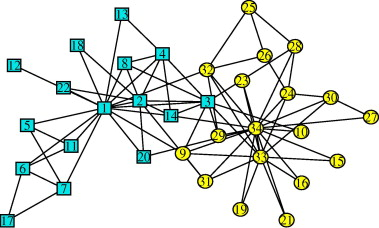
\includegraphics[width=0.5\columnwidth]{./img/karate}%
\caption{Clusters found within Zachary's karate club \cite{zachary77,comellas10}}%
\label{fig:karate}%
\end{figure}

\subsubsection{Clustering}
Within social networks, there are distinct regions of vertices with many connections passing between them, and a much smaller number connected to other vertices outside of this region. These regions are termed as \emph{clusters}.

Social networks are a prime example of this. A person tends to have groups of friends distinct from each other, and friends within these groups are also friends of each other. Figure \ref{fig:socialnetwork} is a social network constructed from data regarding mutual friends of a person. Within this Figure, it can clearly be seen that there exists five distinct regions of mutual friends, with very few links between these regions. These regions are the clusters described above.

With data presented in this manner, it is clear to an observer where these clusters exist, and how many distinct clusters there are. \cite{girvan02} presents an approach to identifying communities within a graph.

\begin{figure}[htbp]
\centering
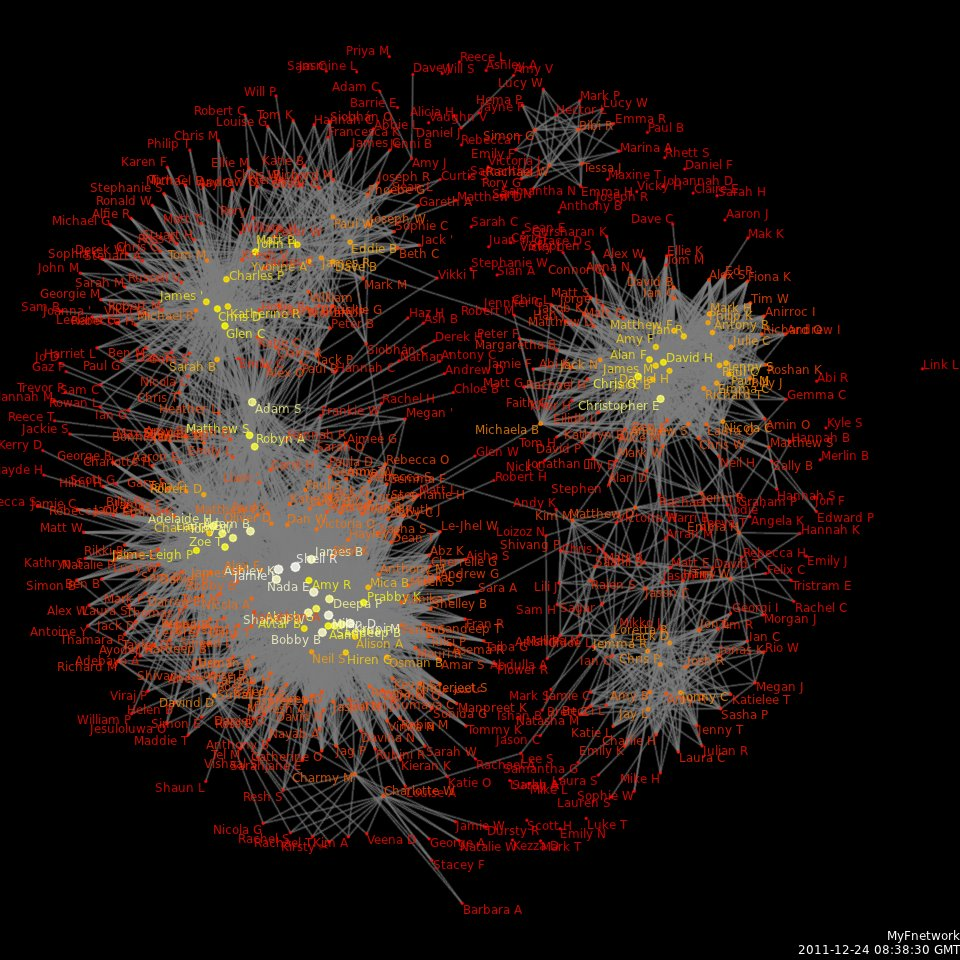
\includegraphics[width=0.5\textwidth]{./img/socialnetwork.png}
\caption{Social Network constructed from Facebook friends using the myFnetwork app}
\label{fig:socialnetwork}
\end{figure}

\subsubsection{Partitioning}
Partitioning of a graph differs from clustering slightly. To partition a graph, we first must know the number of partitions we wish to make, and also the size of each of these partitions. Clustering does not need to know this information as the clusters are produced by the algorithms performing the clustering. Partitioning is related to clustering as it splits the input graph into distinct smaller subgraphs of highly connected vertices, with the subgraphs representing communities within the original graph.

The process of graph partitioning is to divide a graph into smaller parts, such that the number of connections between these smaller parts is as few as possible. The partitions produced are non-overlapping, of a given size, and of a given number.

Graph partitioning is known to be a difficult and complex problem to solve. For simplicity, assume that we are to partition a graph into two partitions. To naively \emph{brute force} all permutations to find the ``best'' partition, which minimises the number of connections between the two partitions, soon becomes unfeasible for anything but the smallest graphs, due to the number of ways of partitioning \emph{n} vertices into two groups \emph{$n_1$} and \emph{$n_2$}. This is $\frac{n!}{n_1!n_2!}$ permutations, and with application of Stirling's formula, can we rewritten as \cite{newman10}:

\begin{equation}
\frac{n!}{n_1!n_2!} \simeq \frac{\sqrt{2\pi n}(n/e)^n}{\sqrt{2\pi n_1}(n_1/e)^{n_1} \sqrt{2\pi n_2}(n_2/e)^{n_2}} = \frac{n^{n+1/2}}{n_1^{n_1+1/2} n_2^{n_2+1/2}} 
\label{eq:partioning1}
\end{equation}

Which, if our two partitions $n_1$ and $n_2$ are equal in size, then the number of permutations of the partition is \cite{newman10}:

\begin{equation}
\frac{n^{n+1/2}}{(n.2)^{n+1}} = \frac{2^{n+1}}{\sqrt{n}}
\label{eq:}
\end{equation}

This shows that running time of the \emph{brute force} algorithm to find all permutations grows exponentially with the size of the input graph.

\citeauthor{kernighan70} proposed an algorithm to solve the partitioning of a graph into two sections \cite{kernighan70}. Initially, the graph is split into two partitions, \emph{A} and \emph{B}. For each pair of vertices (\emph{i, j}) such that $i \in A$ and $j \in B$, the algorithm finds the pair which reduces the number of connections between \emph{A} and \emph{B} the most (see Figure \ref{fig:kernighanlin1}), and swap them (Figure \ref{fig:kernighanlin2}). If there is no pair which reduces the number of connections between the two partitions, then the pair which increases the number of connections by the smallest amount are swapped. This is then repeated until vertices within one partition have been swapped, with the condition that once a vertex has been swapped, it cannot be swapped again. Following this, each state the graph was in after a swap is revisited, with the state with the minimum number of connections between \emph{A} and \emph{B} is minimal. These steps are then repeated until \emph{A} and \emph{B} do not change between rounds. The algorithm has been shown to run in $O(n^2\: log\: n)$ time \cite{kernighan70}, which is marked improvement over the \emph{brute force} $O(2^n)$, but still remains slow and unsuitable for graphs with a over a few thousand vertices \cite{newman10}.

\begin{figure}[htbp]
  \centering
  \subfloat[Original network]{\label{fig:kernighanlin1}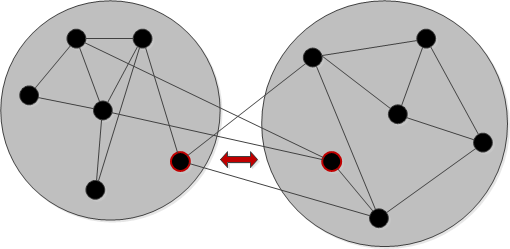
\includegraphics[width=0.3\textwidth]{./img/kernighanlin1}}
  ~ 
  \subfloat[The same network after interchange of two vertices]{\label{fig:kernighanlin2}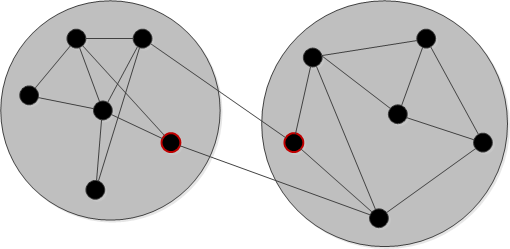
\includegraphics[width=0.3\textwidth]{./img/kernighanlin2}}
  ~ 
  \caption{The Kernighan-Lin algorithm \cite{newman10}}
  \label{fig:kernighanlin}
\end{figure}

Figure \ref{fig:kernighanlin} shows the effect of the Kernigham-Lin algorithm on the original network (Figure \ref{fig:kernighanlin1}). The two vertices highlighted with red reduce the number of connections between the two groups the most, so are swapped. This swap is also the best swap which happens during this iteration of the algorithm, so the network in Figure \ref{fig:kernighanlin2} is selected as the initial network for the next iteration. As no vertex swapping can improve on this, and as such this network is the best network for the next iteration, this network is the solution from the algorithm and the algorithm terminates.

To split a graph into more than two partitions, repeated application of partitioning the subgraphs produced from previous partitioning is applied.

There exist other algorithms to partition graphs, notably spectral algorithms \cite{pothen90,fiedler73}, which make use of properties of the matrix which can be used to define a graph. These spectral algorithms are a lot more complex in the operations needed to execute them, however they operate in $O(n^2)$ time, which is an order $n$ faster than the Kernighan-Lin algorithm \cite{newman10}. It is also noted that spectral algorithms do not necessarily give the best partition, with the partitions produced being of the rough general shape but not quite as good as other algorithms \cite{newman10}.

\subsubsection{\emph{k}-Cliques}
The term \emph{clique} is introduced by \citeauthor{luce49} in \cite{luce49} to describe a subgraph which consists of at least three vertices, each of which are fully connected with each other. From a social network perspective, this translates to saying that for each person in the clique, all of their friends  within the clique are friends of each other as well.

A \emph{k}-clique is defined as a clique which has size \emph{k}. A \emph{maximal clique} is a clique to which no more vertices can be added without violating the conditions of a clique, and the maximum clique is a clique within a graph which contains the largest number of vertices. A 3-clique is also known as a triangle, due to the shape of the graph they are normally represented as (Figure \ref{fig:3clique}).

\begin{figure}[htbp]
\centering
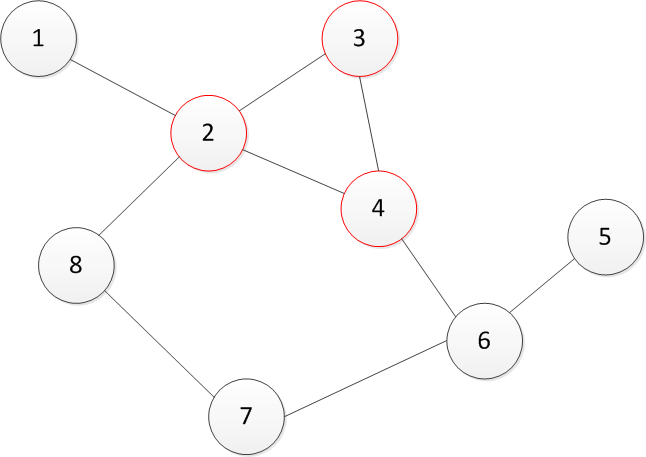
\includegraphics[width=0.5\textwidth]{./img/clique.png}
\caption{Graph highlighting a 3-clique}
\label{fig:clique}
\end{figure}

Figure \ref{fig:clique} shows an example graph highlighting a 3-clique. It has one maximum clique \{2,3,4\} which is highlighted in red, and six other maximal cliques \{1,2\}, \{2,8\}, \{4,6\}, \{5,6\}, \{6,7\}, \{7,8\}.

\begin{figure}
  \centering
  \subfloat[3-clique]{\label{fig:3clique}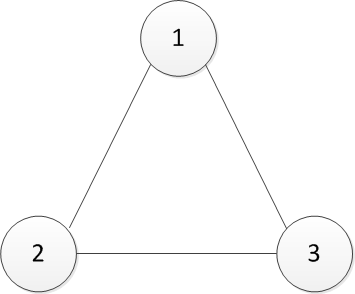
\includegraphics[width=0.3\textwidth]{./img/3-clique}} ~ \subfloat[4-clique]{\label{fig:4clique}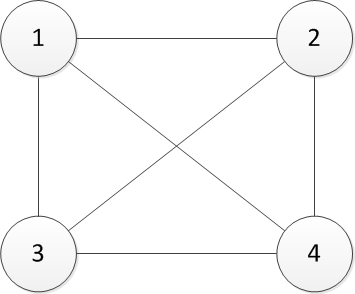
\includegraphics[width=0.3\textwidth]{./img/4-clique}} ~ \subfloat[5-clique]{\label{fig:5clique}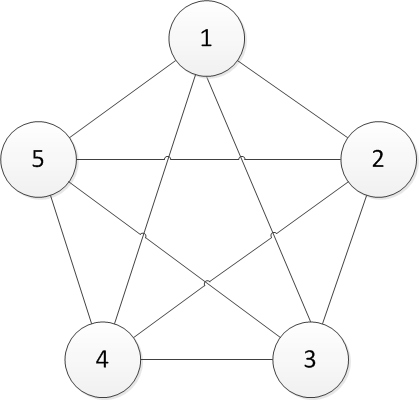
\includegraphics[width=0.3\textwidth]{./img/5-clique}}
  \caption{\emph{k}-cliques}
  \label{fig:cliques}
\end{figure}

Identifying cliques, and solving problems involving cliques as been shown to be computationally hard \cite{bomze99, trusses}. Cliques are either too common, with cliques of only a few members are frequently too numerous to be helpful, or too rare, with large cliques too limiting to be of use \cite{trusses}. Also, computation of identifying cliques scales worse than any polynomial of the problem size, making the process unfeasible for large graphs \cite{trusses, bron72}.

There have been numerous generalisations of the clique construct to improve usefulness of the clique through relaxation of some of the properties of the clique. These include the \emph{n}-clique \cite{luce50}, \emph{n}-clan \cite{alba73} and \emph{n}-club \cite{mokken79}. However these new constructs do not solve the issues of identifying cliques, and remain hard to compute and produce too many results.

\subsubsection{\emph{k}-Trusses}
Following from relaxing properties of the clique, \citeauthor{trusses} in \cite{trusses} introduces a new construct called a truss. A \emph{k}-truss is a subgraph where an edge between two vertices, A and B, exists if at least \emph{k-2} other vertices are connected to both of A and B. The \emph{k}-truss has similar definitions to the clique. A maximal \emph{k}-truss is a \emph{k}-truss that is not a proper subgraph of another \emph{k}-truss.

\begin{figure}[htbp]
\centering
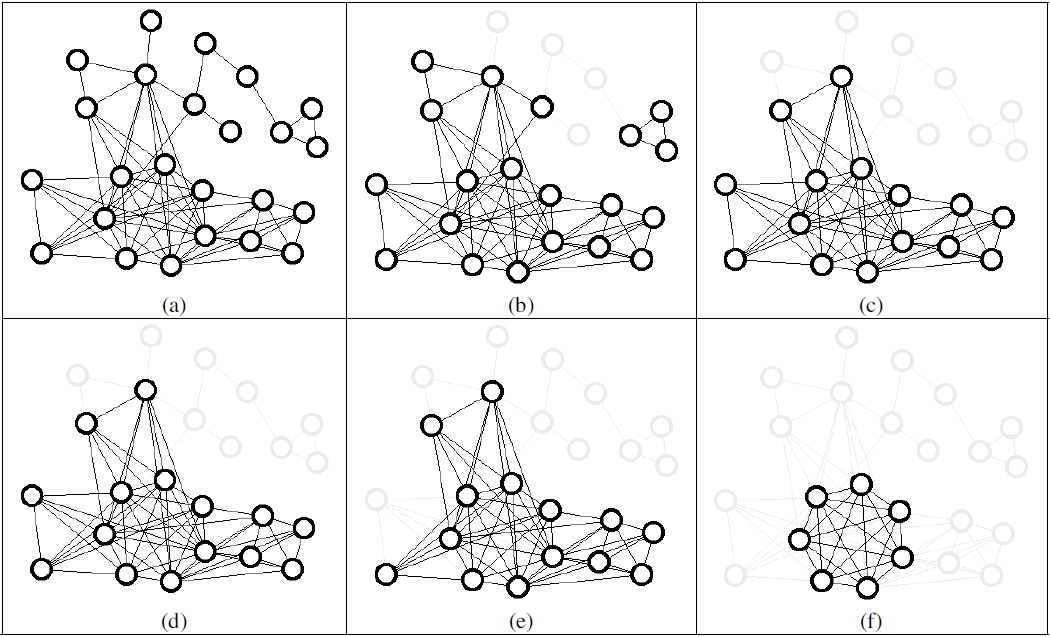
\includegraphics[width=0.9\textwidth]{./img/trusses.png}
\caption{An Example of Maximal Trusses. (a) original graph, (b) 3-trusses, (c) 4-truss, (d) 5-truss, (e) 6-truss. Note that (c) and (d) are the same. \cite{trusses}}
\label{fig:trusses}
\end{figure}

Figure \ref{fig:trusses} shows an example application of \emph{k}-trusses. Figure \ref{fig:trusses}(a) shows the original graph. Figures \ref{fig:trusses}(b-f) show the \emph{k}-truss for increasing values of \emph{k}. If the same original graph were to be analysed for \emph{k}-cliques for the same values of \emph{k}, more vertices in the graph would have been removed in earlier stages, which would have lost the interesting stage where Figures \ref{fig:trusses}(c) and (d) are identical.

The \emph{k}-truss is also computable in polynomial time to the input graph, which offers a marked improvement on the computation costs of identifying cliques and similar constructs. \cite{trusses} shows that the naive algorithm  for computing maximal \emph{k}-trusses is bounded by $O(n|E|^2 + n)$, where \emph{n} is the number of vertices in the graph, and \emph{|E|} is the number of edges in the graph. A more efficient method is shown to take $O(\Sigma d^2(v))$, where \emph{d(v)} is the degree of a vertex, \emph{v}.
